\chapter{Séries temporais}
\label{chap:time-series}
Na área médica, é comum a monitoração da evolução de funções vitais de pacientes através de aparelhos como eletroencefalogramas e eletrocardiogramas, além do acompanhamento da incidência de padrões sazonais de epidemias~\cite{metodosmedicina}. Na ciência econômica, muitos livros~\cite{forecastingeconomic} e artigos~\cite{germantimeseries} já foram escritos sobre análises e previsões do mercado financeiro, políticas fiscais e monetárias, baseadas em observações no tempo. O que a Medicina e a Economia e outras áreas supostamente não correlatas possuem em comum é o fato de permitirem a aplicação de estudos e métodos de séries temporais.

Séries temporais podem ser construídas sobre praticamente quaisquer medições possíveis no tempo e esse caráter genérico é o que torna a utilidade do seu estudo indiscutível em diversas áreas do conhecimento humano. O tema é usado com sutis diferenças entre matemáticos, estatísticos e outros profissionais. Por essa razão, segue a definição que será utilizada\footnote{Séries temporais também podem ser definidas como um conjunto de observações $\{X(t), t \in T\}$, com $X$ representando a variável aleatória observada e T um conjunto de índices.}:


\theoremstyle{definition}
\newtheorem{time-series}{Definição}
\begin{time-series}
Série temporal: sequência de observações\footnote{Tais observações podem ser coletadas em períodos regulares ou não.} ordenadas cronologicamente (n-tupla):
\begin{equation}\label{eq:time-series}
 \\S = (s_{1}, s_{2}, s_{3}, ..., s_{n})
\end{equation}
\end{time-series}

  \begin{figure}
    \begin{center}
      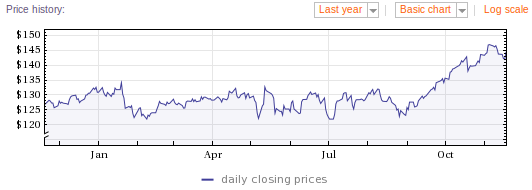
\includegraphics[width=0.9\textwidth]{ibm_stock}
      \centering
      \caption[Preço de fechamento de ações da IBM - 2010.]{Preço de fechamento de ações da IBM no ano de 2010~\cite{wolframalpha}.}
    \label{fig:ibm-stock}
    \end{center}
  \end{figure}

Quando tais observações são coletadas no tempo continuamente, diz-se que a série temporal é \textit{contínua} e quando as medições se fazem em instantes de tempo específicos, geralmente equidistantes, são conhecidas como séries temporais \textit{discretas}. 

Na figura \ref{fig:ibm-stock}, podemos visualizar um exemplo de série temporal discreta, descrevendo o preço de fechamento das ações da IBM ao longo do ano de 2010.

Em geral, o estudo de séries temporais comporta objetivos dos mais diversos, como identificação de tendências e outliers\footnote{Observações distantes ou discrepantes quando comparadas globalmente com outras observações.}, predição, similaridade entre séries temporais por clusterização, existência de sazonalidades -- endereçado na seção \ref{sub:sazonalidade} -- entre outros.

A seguir, serão apresentadas características e técnicas envolvidas na visualização, representação e análise de séries temporais. Ao final deste capítulo, contextualizaremos o papel de séries temporais com a realidade de grandes datacenters.

\section{Características}
\subsection{Dependência de observações}
O valor das ações da IBM ao final de um dia se torna naturalmente dependente do seu desempenho em dias anteriores. Da mesma forma, o número de pessoas que habitavam o planeta Terra em anos passados tem influência direta sobre a população mundial de hoje.

É comum encontrar na literatura~\cite{timeseriesr}, ressalvas sobre a aplicação de muitos métodos estatísticos tradicionalmente baseados na suposição de que observações adjacentes são independentes e identicamente distribuídas. Sendo assim, identificar a existência de correlações entre medições no tempo é essencial para que possamos aplicar análises estatísticas apropriadas.

\subsection{Alta dimensionalidade}
\label{sub:alta-dimensionalidade}
É comum observar na literatura a interpretação da n-tupla descrita na definição \ref{eq:time-series} como um ponto em uma espaço de dimensão $\Re^n$. Como novas observações são coletadas constantemente, séries temporais assumem, portanto, caráter de alta dimensionalidade.

Como possuem centenas de milhares a milhões de pontos e tratá-los em sua forma bruta se torna computacionalmente custoso, é desejável, em aplicações práticas, um mecanismo que favoreça a redução de dimensionalidade.

\subsection{Sazonalidade}
\label{sub:sazonalidade}
É possível identificar na Natureza diversos fenômenos que possuem algum comportamento sazonal. A produção de arroz na China, o número de passagens vendidas por uma companhia aérea ao longo de um ano, a migração das aves com a chegada do inverno e a quantidade de visitas em uma página na Internet possuem no mínimo um comportamento em comum: sazonalidade.

No contexto de séries temporais, o termo \textit{sazonalidade} diz respeito a padrões que se repetem em períodos no tempo. Sazonalidades podem ser classificadas em dois tipos: aditivas e multiplicativas. A primeira retrata flutuações que não sofrem mudanças muito bruscas quando considerada a série globalmente. Sazonalidades multiplicativas dependem de um fator em cada período em que é observada e possuem uma maior variabilidade quando comparadas com a série original como um todo.

\subsection{Tendência}
A quantidade de água doce no mundo vem diminuindo ao longo dos anos. Ao mesmo tempo, o número de artigos científicos publicados no meio acadêmico cresce monotonicamente. Tendências de crescimento ou decrescimento podem ser identificadas em séries temporais e podem ser caracterizadas por sua taxa de variação. Se sua taxa de crescimento se aproximar de uma reta, diz-se que a série possui tendência linear. Caso contrário, tendências podem ser classificadas como não lineares, exponenciais ou quadráticas.


\begin{figure}[htb!]
  \begin{center}
    \subfloat[Sem tendência ou sazonalidade]{\label{fig:ts0}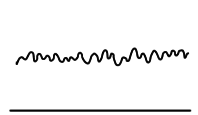
\includegraphics[width=0.25\textwidth]{tend-sazonalidade0}} \quad
    \subfloat[Sem tendência, com sazonalidade]{\label{fig:ts1}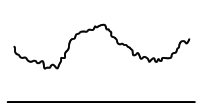
\includegraphics[width=0.25\textwidth]{tend-sazonalidade1}} \quad
    \subfloat[Tendência linear, com sazonalidade aditiva]{\label{fig:ts2}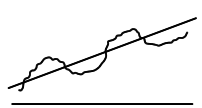
\includegraphics[width=0.25\textwidth]{tend-sazonalidade2}}
    \\
    \subfloat[Tendência linear e sazonalidade multiplicativa]{\label{fig:ts3}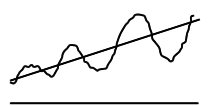
\includegraphics[width=0.25\textwidth]{tend-sazonalidade3}} \quad
    \subfloat[Tendência não linear e sazonalidade aditiva]{\label{fig:ts4}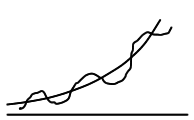
\includegraphics[width=0.25\textwidth]{tend-sazonalidade4}} \quad
    \subfloat[Tendência não linear e sazonalidade multiplicativa]{\label{fig:ts5}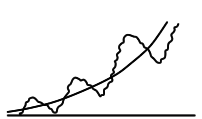
\includegraphics[width=0.25\textwidth]{tend-sazonalidade5}}
    \centering
    \caption{Padrões de tendência e sazonalidade em séries temporais}
  \label{fig:tend-sazonalidade}
  \end{center}
\end{figure}

Na figura \ref{fig:tend-sazonalidade}, padrões de comportamento relacionando sazonalidade e tendência podem ser observados. Além das características apresentadas, outras bastante utilizadas na literatura e não menos importantes são  estacionariedade, aleatoriedade e ciclidade. A seguir, uma breve descrição de técnicas largamente utilizadas para análise e compressão de séries temporais.

\section{Representação e redução de dimensionalidade}
A representação de séries temporais em sua forma original pode ser computacionalmente custosa, dada sua alta dimensionalidade -- discutida na seção \ref{sub:alta-dimensionalidade}. A escolha do método de representação deve se basear na aplicabilidade desejada. Existem atualmente diversas abordagens para compressão e representação de séries temporais. Algumas se baseiam em transformações de domínios, como \textit{Discrete Fourier Transform}, que mapeiam para o domínio de frequências uma série em seu domínio temporal, outras podem preservar dois domínios, como é o caso de \textit{Discrete Wavelet Transform}. O objetivo dessa seção é apresentar as ideias das abordagens mais conhecidas e utilizadas.

\subsection{Algoritmos utilizados}
Séries temporais podem ser vistas como funções matemáticas e como tais podem se favorecer de técnicas básicas da Matemática Aplicada, como aproximações de funções complexas por funções mais simples, como retas. O método conhecido como PLA (Piecewise Linear Approximation) segmenta uma série temporal em partes e para cada uma delas define a reta que mais se aproxima dos pontos no segmento considerado. Na figura \ref{fig:pla} podemos ver um exemplo de como uma série pode ser aproximada por esse método.

  \begin{figure}[htb!]
    \begin{center}
      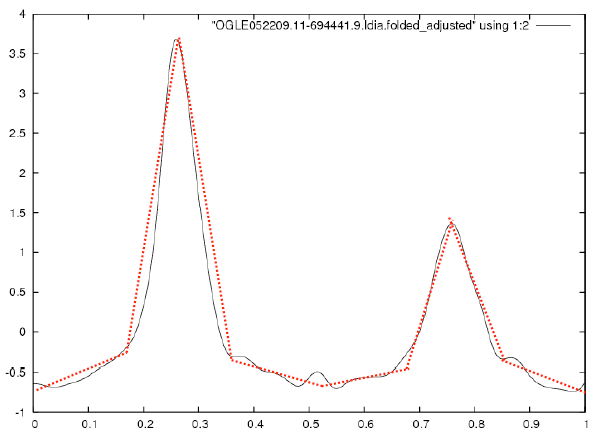
\includegraphics[width=0.6\textwidth]{pla}
      \centering
      \caption{Piecewise Linear Approximation}
    \label{fig:pla}
    \end{center}
  \end{figure}

Abordagens com teor matemático mais apurados também são utilizadas para representar séries temporais. Os resultados de Jean-Baptiste Joseph Fourier, que demonstrou que todo sinal periódico poderia ser aproximado por somas de senos e cossenos, podem ser mapeados para o campo dos números complexos, dando origem a transformada de Fourier.

  \begin{figure}[htb!]
    \begin{center}
      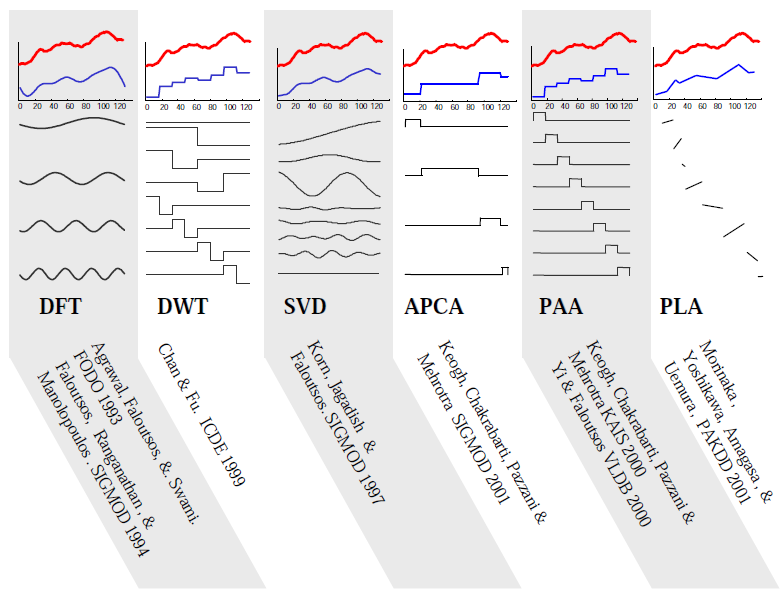
\includegraphics[width=1\textwidth]{comparing_methods}
      \centering
      \caption[Comparação entre algoritmos de representação.]{Comparação entre algoritmos de representação e redução de dimensionalidade de séries temporais.}
    \label{fig:comparing-methods}
    \end{center}
  \end{figure}

A partir dessa transformada, uma série temporal pode ser decomposta por suas componentes no domínio das frequências. Na primeira coluna da figura \ref{fig:comparing-methods} podemos ver como uma aproximação pode ser feita com o algoritmo FFT (Fast Fourier Transform), uma das variantes de uma classe maior de algoritmos baseados na transformada de Fourier, conhecida como DFT (Discrete Fourier Transform). Uma desvantagem deste método é que se perde o referencial de eventos no tempo, tendo que se recorrer a transformada inversa de Fourier~\cite{dftandwavelets}.

Outro algoritmo largamente utilizado para compressão de imagens e que pode ser utilizado para redução de dimensionalidade de séries temporais é o DWT (Discrete Wavelet Transform), mais vantajoso do que o DFT em alguns aspectos, pois preserva componentes no domínio do tempo~\cite{insightintowavelets}. Uma ``wavelet'' ou ondaleta é uma pequena onda que pode ser usada como base para a reconstrução da série original e diferente dos senos e cossenos utilizados no DFT não podem ser funções periódicas. Para a utilização desse algoritmo é necessário que se escolha previamente duas ondaletas, normalmente conhecidas como ondas mãe $\psi$ e pai $\phi$ que devem satisfazer alguns critérios de ortogonalidade. 

  \begin{figure}[htb!]
    \begin{center}
      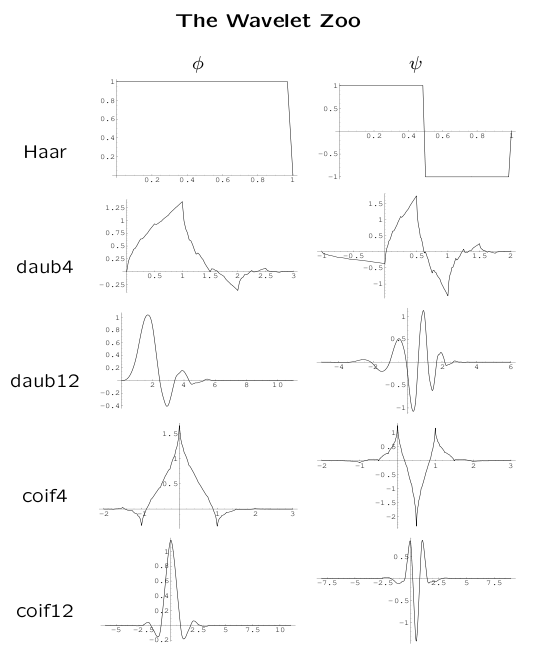
\includegraphics[width=0.7\textwidth]{zoo}
      \centering
      \caption{Família de Wavelets.}
    \label{fig:zoo}
    \end{center}
  \end{figure}



Na figura \ref{fig:zoo} podemos ver pares de funções mãe e pai que satisfazem esses critérios e podem ser utilizadas como wavelets. Repare na segunda coluna da figura \ref{fig:comparing-methods} a aproximação de uma série utilizando a ondaleta Haar, reconhecida como a primeira ondaleta utilizada.

Ainda na figura \ref{fig:comparing-methods}, pode-se observar como os métodos apresentados e outros se comportam para a mesma série original de entrada. Em cada coluna, a série original de entrada aparece em vermelho e logo abaixo, em azul, a série aproximada pelo algoritmo correspondente. Comparações mais detalhadas sobre DFT e DWT podem ser encontradas em~\cite{dftandwavelets}.

Além dos apresentados, existem na literatura diversos algoritmos de representação e redução de dimensionalidade de séries temporais. Alguns deles são: Piecewise Constant Approximation (PCA), Symbolic Approximation (SA), Symbolic Aggregate ApproXimation (SAX), Singular Value Decomposition (SVD), CHEByshev polynomials (CHEB) e Self-Organizing Maps (SOM).

A partir dessa visão geral sobre o atual cenário no que diz respeito a representação e compressão de séries temporais, na próxima seção uma contextualização com o ambiente de datacenters será apresentada.

\section{Séries temporais de datacenters}
\label{sec:time-series-datacenter}
Datacenters são ambientes que concentram equipamentos de processamento e armazenamento de dados de empresas ou organizações. Podem ser considerados como legítimas ``máquinas'' de produção de séries temporais. Em uma instalação típica, são encontrados diversos racks de servidores centralizadores de inúmeras unidades de processamento e armazenamento.

O foco deste trabalho se concentra em séries temporais de observações feitas sobre os equipamentos e dispositivos desses datacenters. O operador de um grande datacenter, em geral, precisa monitorar dados de consumo de CPU, memória, sessões TCP abertas, requisições HTTP, taxa de hits em caches, número de consultas lentas a bancos de dados, entre outras métricas. Em datacenters possuímos um conjunto bem heterogêneo de padrões de séries temporais. Na figura \ref{fig:series-temporais-datacenter} podemos ver alguns exemplos de gráficos que fazem parte do dia a dia de operação de um datacenter. 

Esses gráficos foram gerados através de uma ferramenta bem conhecida, RRDtool. Com essa ferramenta é possível escrever scripts para coletar informações de dispositivos de tempos em tempos. O software é livre e utiliza o conceito de Round Robin Database, em que é mantido sempre uma quantidade fixa de pontos de cada série. Quando o limite é ultrapassado, algumas estratégias podem ser definidas. A mais simples de todas é descartar sempre os pontos mais antigos. Pode-se também configurar cálculos de agregados, resumindo pontos por sua média, mínimo ou máximo. 

Essa abordagem nem sempre é satisfatória na busca por uma causa para uma possível falha em um desses equipamentos, pois médias em dados com variância muito alta podem mascarar falhas graves. É desejável, portanto, que se tenha uma forma eficiente de visualização que permita capturar características apresentadas nesse capítulo, como sazonalidades e tendências. Essas observações é que permitirão coletar fatos e reorganizar a estrutura do datacenter para que o mesmo se mantenha em pleno funcionamento. Para tanto, algum dos algoritmos de representação e redução de dimensionalidade se faz necessário. 

No próximo capítulo veremos as ideias que estão por trás do algoritmo \textit{Perceptually Important Points}, seguido de sua implementação e a contextualização com datacenters será retomada no capítulo \ref{chap:holmes}, que retratará a aplicação do algoritmo em um sistema real de monitoração.

\begin{figure}[htb!]
  \begin{center}
    \subfloat[Consumo de CPU]{\label{fig:cpu}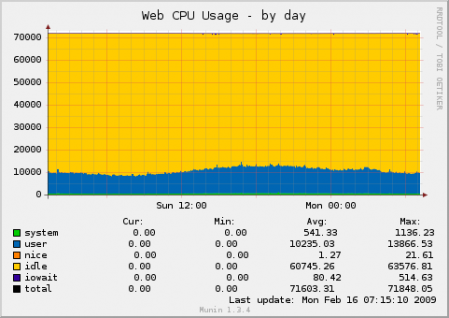
\includegraphics[width=0.7\textwidth]{cpu}}
    \\
    \subfloat[Tráfego de rede]{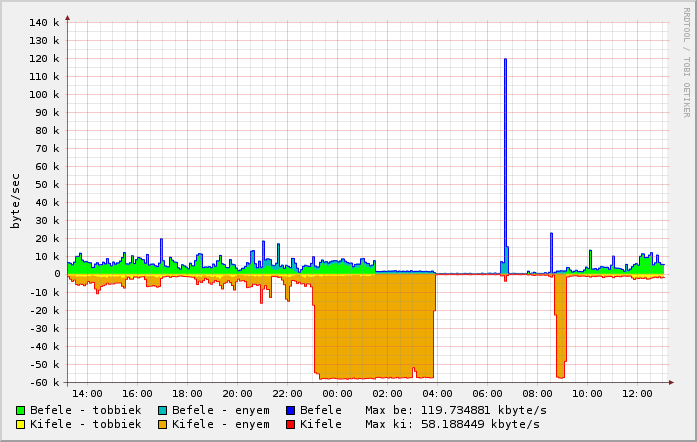
\includegraphics[width=0.7\textwidth]{network_day}}
    \\
    \subfloat[Uso do protocolo SMPP em um roteador]{\label{fig:pip2}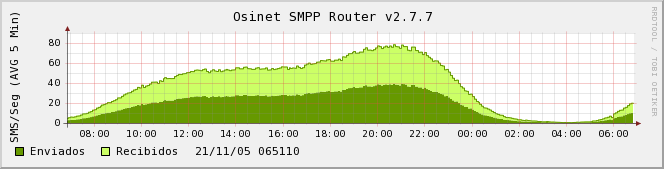
\includegraphics[width=0.7\textwidth]{smpp_router}}
    \\
    \centering
    \caption{Gráficos típicos no dia a dia de operação de um datacenter}
    \label{fig:series-temporais-datacenter}
  \end{center}
\end{figure}

